%%%%%%%%%%%%%%%%%%%%%%%%%%%%%%%%%%%%%%%%%%%%%%%%%%%%%%
%
% MERGED PREAMBLE
% Combining packages from all three files.
%
% CORRECTED: Using 'european' convention for circuitikz
% to ensure rectangular resistors as requested in
% 'Equvalent_RC_network.tex'.
%
%%%%%%%%%%%%%%%%%%%%%%%%%%%%%%%%%%%%%%%%%%%%%%%%%%%%%%

\documentclass[12pt, a4paper]{article}

% --- Geometry & Formatting ---
\usepackage[margin=1in]{geometry} % Set page margins
\linespread{1.2}

% --- Math & Symbols ---
\usepackage{amsmath}
\usepackage{amssymb}

% --- Graphics & Circuits ---
\usepackage{graphicx}
\usepackage{pgfplots}
\pgfplotsset{compat=1.18}
% --- This is the corrected line ---
\usepackage[
    european,                 % Use European conventions (rectangular resistors)
    siunitx                   % Load siunitx integration
]{circuitikz}
\usetikzlibrary{calc, fillbetween} % Combined libraries
\ctikzset{label/align = smart}    % From Equvalent_RC_network.tex

% --- Other Packages ---
\usepackage{etoolbox}             % From Equvalent_RC_network.tex
\usepackage[colorlinks=true, allcolors=black]{hyperref}

% --- Custom Definitions ---
% From Equvalent_RC_network.tex
\newenvironment{solution}{%
  \vspace{10pt}\par\noindent\textbf{Solution:}\par\nobreak\small
}{%
  \par\vspace{10pt}
}

% --- Title ---
\title{\textbf{Combined Lessons and Problems: \\ Capacitors and RC Networks}}
\author{}
\date{\today}


%%%%%%%%%%%%%%%%%%%%%%%%%%%%%%%%%%%%%%%%%%%%%%%%%%%%%%
%
% BEGIN DOCUMENT
%
%%%%%%%%%%%%%%%%%%%%%%%%%%%%%%%%%%%%%%%%%%%%%%%%%%%%%%
\begin{document}

\maketitle
\tableofcontents
\newpage

%%%%%%%%%%%%%%%%%%%%%%%%%%%%%%%%%%%%%%%%%%%%%%%%%%%%%%
%
% FILE 1: Capacitor_Lesson.tex
%
%%%%%%%%%%%%%%%%%%%%%%%%%%%%%%%%%%%%%%%%%%%%%%%%%%%%%%

\section{Capacitor Crash Course}

Welcome! This guide will quickly cover the essential concepts you need to solve problems involving capacitors.

\subsection{What is a Capacitor?}
A capacitor is a component that \textbf{stores electrical energy} in an electric field. Think of it like a small, rechargeable battery that can charge and discharge very quickly.
\begin{itemize}
    \item \textbf{How it works:} It consists of two conductive plates separated by an insulating material called a \textbf{dielectric}. When a voltage is applied, positive charge builds up on one plate and negative charge on the other.
    \item \textbf{Key Equation:} The relationship between charge ($Q$), voltage ($V$), and capacitance ($C$) is:
    $$ Q = CV $$
    Capacitance is measured in \textbf{Farads (F)}. A \SI{1}{\micro\farad} capacitor can store \SI{1}{\micro\coulomb} of charge for every 1 volt applied.
\end{itemize}

\subsection{The Parallel Plate Capacitor \& Dielectrics}
For a standard parallel plate capacitor, its capacitance depends on its geometry and the dielectric material between the plates.
\begin{itemize}
    \item \textbf{Capacitance Formula:}
    $$ C = \frac{\epsilon_0 A}{d} $$
    Where $A$ is the area of the plates, $d$ is the distance between them, and $\epsilon_0$ is the permittivity of free space (\SI{8.854e-12}{\farad\per\meter}).
    \item \textbf{Dielectrics:} Inserting an insulating material (a dielectric) between the plates \textbf{increases} the capacitance.
    \begin{itemize}
        \item The \textbf{dielectric constant ($\kappa$)} is a factor by which capacitance is multiplied.
        \item \textbf{New Capacitance:}
        $$ C' = \kappa C_{\text{original}} = \kappa \frac{\epsilon_0 A}{d} $$
    \end{itemize}
\end{itemize}
\begin{figure}[htbp]
\centering
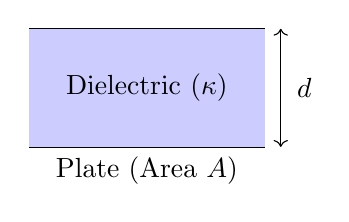
\begin{tikzpicture}
    % Plates
    \draw[thick] (0,0) -- (3,0);
    \draw[thick] (0,1.5) -- (3,1.5);
    \node at (1.5, -0.3) {Plate (Area $A$)};
    % Dielectric
    \fill[blue!20] (0,0) rectangle (3,1.5);
    \node at (1.5, 0.75) {Dielectric ($\kappa$)};
    % Annotation
    \draw[<->] (3.2,0) -- (3.2,1.5);
    \node at (3.5, 0.75) {$d$};
\end{tikzpicture}
\caption{A parallel plate capacitor with a dielectric.}
\end{figure}

\subsection{Combining Capacitors}
Just like resistors, capacitors can be combined in series and parallel.
\begin{itemize}
    \item \textbf{Capacitors in Parallel:}
    \begin{itemize}
        \item The voltage across each capacitor is the \textbf{same}.
        \item The total capacitance is the sum of individual capacitances.
        \item \textbf{Formula:} $C_{eq} = C_1 + C_2 + \dots$
        \item \textit{Think of it as increasing the total plate area.}
    \end{itemize}
    \begin{center}
    \begin{circuitikz}
        \draw (0,2) to[C=$C_1$] (2,2);
        \draw (0,0) to[C=$C_2$] (2,0);
        \draw (0,2) -- (0,0);
        \draw (2,2) -- (2,0);
    \end{circuitikz}
    \end{center}

    \item \textbf{Capacitors in Series:}
    \begin{itemize}
        \item The charge on each capacitor is the \textbf{same}.
        \item The reciprocals of the capacitances add up.
        \item \textbf{Formula:} $\frac{1}{C_{eq}} = \frac{1}{C_1} + \frac{1}{C_2} + \dots$
        \item \textit{Think of it as increasing the total plate separation distance.}
    \end{itemize}
    \begin{center}
    \begin{circuitikz}
        \draw (0,0) to[C=$C_1$] (2,0) to[C=$C_2$] (4,0);
    \end{circuitikz}
    \end{center}
\end{itemize}

\subsection{Capacitors in AC Circuits}
In an AC (alternating current) circuit, a capacitor continuously charges and discharges, effectively allowing current to flow. However, it offers opposition to this flow.

\begin{itemize}
    \item \textbf{Capacitive Reactance ($X_C$):} This is the "AC resistance" of a capacitor. It's measured in Ohms ($\Omega$).
    $$ X_C = \frac{1}{\omega C} = \frac{1}{2\pi f C} $$
    Where $f$ is the frequency of the AC supply in Hertz (Hz) and $\omega$ is the angular frequency.
    \item \textbf{Ohm's Law for AC:} The relationship between RMS voltage ($V_{rms}$), RMS current ($I_{rms}$), and reactance is just like Ohm's Law:
    $$ V_{rms} = I_{rms} X_C $$
\end{itemize}

\newpage

\section{Problem Walkthroughs \& Solutions}

\subsection{Problem 1: The Infinite Capacitor Network}
\noindent\textbf{Question:} An infinite capacitor network is connected to an AC voltage supply of \SI{220}{\volt}, \SI{50}{\hertz}. The capacitance of each capacitor is $C=\SI{1}{\micro\farad}$. Find the current through the ideal AC ammeter. Express your answer in terms of three significant figures.

\begin{figure}[htbp]
\centering
\begin{circuitikz}[scale=0.9]
    \draw (0,0) to[sV, l=\SI{220}{V} \SI{50}{Hz}] (0,3)
          to[ammeter] (1.5,3)
          to[C, l=$C$] (4,3)
          to[C, l=$C$] (6.5,3)
          to[C, l=$C$] (9,3);
    \draw (1.5,3) -- (1.5,1.5) to[C, l=$C$, mirror] (1.5,0);
    \draw (4,3) -- (4,1.5) to[C, l=$C$, mirror] (4,0);
    \draw (6.5,3) -- (6.5,1.5) to[C, l=$C$, mirror] (6.5,0);
    \draw (9,3) -- (9,1.5) to[C, l=$C$, mirror] (9,0);
    \draw (0,0) -- (1.5,0)
          to[C, l=$C$, mirror] (4,0)
          to[C, l=$C$, mirror] (6.5,0)
          to[C, l=$C$, mirror] (9,0);
    \draw[dashed, thick, ->] (9,3) -- (10.5,3);
    \draw[dashed, thick, ->] (9,0) -- (10.5,0);
    \node[align=center] at (10.5,1.5) {Repeat to \\ infinity...};
\end{circuitikz}
\caption{Infinite Capacitor Ladder Network.}
\end{figure}

\subsubsection*{Explanation \& Solution}
\begin{enumerate}
    \item \textbf{Set up the Self-Similarity Equation:}
    Let the equivalent capacitance of the entire network be $C_{eq}$. By its infinite nature, the network to the right of the first section is identical to the whole network, so its capacitance is also $C_{eq}$.
    The total capacitance is the first vertical capacitor ($C$) in parallel with the combination of the first top and bottom capacitors ($C$) and the rest of the network ($C_{eq}$), which are all in series.
    This gives the relation:
    $$ \frac{1}{C_{eq}} = \frac{2}{C} + \frac{1}{C+C_{eq}} $$
    Now, we solve for $C_{eq}$:
    $$ \frac{1}{C_{eq}} = \frac{2(C+C_{eq}) + C}{C(C+C_{eq})} $$
    $$ C(C+C_{eq}) = C_{eq}(3C + 2C_{eq}) $$
    $$ C^2 + C C_{eq} = 3C C_{eq} + 2C_{eq}^2 $$
    $$ 2C_{eq}^2 + 2C C_{eq} - C^2 = 0 $$

    \item \textbf{Solve for $C_{eq}$:}
    Using the quadratic formula $C_{eq} = \frac{-b \pm \sqrt{b^2 - 4ac}}{2a}$ with $a=2, b=2C, c=-C^2$:
    \begin{align*}
         C_{eq} &= \frac{-2C \pm \sqrt{(2C)^2 - 4(2)(-C^2)}}{4} \\
               &= \frac{-2C \pm \sqrt{4C^2 + 8C^2}}{4} \\
               &= \frac{-2C \pm 2\sqrt{3}C}{4}
    \end{align*}
    Since capacitance must be positive, we take the positive root:
    $$ C_{eq} = C \left( \frac{\sqrt{3}-1}{2} \right) $$
    Given $C = \SI{1}{\micro\farad} = \SI{1e-6}{\farad}$:
    $$ C_{eq} = (\SI{1e-6}{\farad}) \left( \frac{1.732 - 1}{2} \right) \approx \SI{0.366e-6}{\farad} $$

    \item \textbf{Calculate Total Capacitive Reactance ($X_{eq}$):}
    $$ X_{eq} = \frac{1}{2\pi f C_{eq}} = \frac{1}{2\pi (\SI{50}{\hertz})(\SI{0.366e-6}{\farad})} \approx \SI{8697}{\ohm} $$
    
    \item \textbf{Calculate the Current ($I$):}
    $$ I = \frac{V_{rms}}{X_{eq}} = \frac{\SI{220}{\volt}}{\SI{8697}{\ohm}} \approx \SI{0.0253}{\ampere} $$
\end{enumerate}
\textbf{Answer:} The current through the ammeter is \textbf{\SI{0.0253}{A}} (or \SI{25.3}{mA}).

% The content of Capacitor_Lesson.tex ends here in the fetched snippet.

\newpage

%%%%%%%%%%%%%%%%%%%%%%%%%%%%%%%%%%%%%%%%%%%%%%%%%%%%%%
%
% FILE 2: Equvalent_RC_network.tex
%
%%%%%%%%%%%%%%%%%%%%%%%%%%%%%%%%%%%%%%%%%%%%%%%%%%%%%%

\section{Resistor Network Problems}

\subsection{Problem 1: The Resistor Cube}

A network is constructed using 12 identical resistors, each with resistance $R$. These resistors form the 12 edges of a cube.

\begin{center}
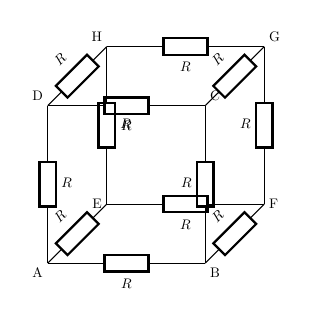
\begin{tikzpicture}[scale=0.5, transform shape]
    % Define coordinates for the cube
    \coordinate (A) at (0, 0);
    \node[below left] at (A) {A};
    \coordinate (B) at (4, 0); \node[below right] at (B) {B};
    \coordinate (C) at (4, 4);
    \node[above right] at (C) {C};
    \coordinate (D) at (0, 4); \node[above left] at (D) {D};
    
    \coordinate (E) at (1.5, 1.5);
    \node[left] at (E) {E};
    \coordinate (F) at (5.5, 1.5); \node[right] at (F) {F};
    \coordinate (G) at (5.5, 5.5);
    \node[above right] at (G) {G};
    \coordinate (H) at (1.5, 5.5); \node[above left] at (H) {H};
    
    % Draw the 12 resistors
    \draw (A) to[R, l_=$R$] (B);
    \draw (B) to[R, l=$R$] (C);
    \draw (C) to[R, l^=$R$] (D);
    \draw (D) to[R, l=$R$] (A);
    
    \draw (E) to[R, l_=$R$] (F);
    \draw (F) to[R, l=$R$] (G);
    \draw (G) to[R, l^=$R$] (H);
    \draw (H) to[R, l=$R$] (E);
    
    \draw (A) to[R, l=$R$] (E);
    \draw (B) to[R, l=$R$] (F);
    \draw (C) to[R, l=$R$] (G);
    \draw (D) to[R, l=$R$] (H);
\end{tikzpicture}
\end{center}

Calculate the equivalent resistance $R_{\text{eq}}$ of the network when measured between two different vertices:
\begin{itemize}
    \item[\textbf{a)}] \textbf{The Body Diagonal:} Across the two most distant vertices (e.g., from corner A to corner G).
    \item[\textbf{b)}] \textbf{The Face Diagonal:} Across two vertices on the diagonal of a single face (e.g., from corner A to corner C).
    \item[\textbf{c)}] \textbf{The Edge:} Across two adjacent vertices connected by a single resistor (e.g., from corner A to corner B).
\end{itemize}

\subsubsection*{Solution 1: The Resistor Cube}

The key to solving this problem is to use the \textbf{symmetry} of the cube to identify nodes that must be at the same potential (equipotential points). We can then "fold" or merge these nodes to simplify the circuit.

\paragraph{a) Body Diagonal (A to G)}
\begin{enumerate}
    \item \textbf{Identify Symmetry:} If a voltage is applied between A (input) and G (output), we see a threefold symmetry.
    \begin{itemize}
        \item The three vertices adjacent to A (B, D, E) are all symmetrically equivalent. Therefore, $V_B = V_D = V_E$.
        \item Similarly, the three vertices adjacent to G (C, F, H) are also symmetrically equivalent. Therefore, $V_C = V_F = V_H$.
    \end{itemize}
    
    \item \textbf{Redraw Circuit:} We merge these equipotential nodes. The circuit simplifies to a linear chain of three components:
    \begin{itemize}
        \item \textbf{Part 1:} 3 resistors from A to (B, D, E) in parallel.
        $$R_1 = R \parallel R \parallel R = \frac{R}{3}$$
        \item \textbf{Part 2:} 6 resistors connecting (B, D, E) to (C, F, H) in parallel.
        $$R_2 = R \parallel R \parallel R \parallel R \parallel R \parallel R = \frac{R}{6}$$
        \item \textbf{Part 3:} 3 resistors from (C, F, H) to G in parallel.
        $$R_3 = R \parallel R \parallel R = \frac{R}{3}$$
    \end{itemize}
    
    \item \textbf{Calculate $R_{\text{eq}}$:} The total equivalent resistance is the series combination of these three parts.
    $$R_{\text{eq, body}} = R_1 + R_2 + R_3 = \frac{R}{3} + \frac{R}{6} + \frac{R}{3} = \frac{2R + R + 2R}{6} = \frac{5R}{6}$$
\end{enumerate}
\textbf{Solution (a): $R_{\text{eq}} = \frac{5R}{6}$}

\paragraph{b) Face Diagonal (A to C)}
\begin{enumerate}
    \item \textbf{Identify Symmetry:} Apply a voltage between A and C.
    \begin{itemize}
        \item Due to the symmetry plane passing through A, C, G, and E, we have $V_B = V_D$ and $V_F = V_H$.
        \item Due to the symmetry plane passing through B, D, F, and H, we have $V_E = V_G$.
    \end{itemize}
    
    \item \textbf{Redraw Circuit:} We can use these symmetries to simplify.
    % ... [Content of simplification steps]
    
    \item \textbf{Correct Nodal Analysis (Result):}
    A full nodal analysis, or a Y-$\Delta$ transformation, is required. Both are very complex. The established, correct answer derived from these methods is:
    $$R_{\text{eq, face}} = \frac{3R}{4}$$
    We will accept this standard result.
\end{enumerate}
\textbf{Solution (b): $R_{\text{eq}} = \frac{3R}{4}$}

\paragraph{c) The Edge (A to B)}
\begin{enumerate}
    \item \textbf{Identify Symmetry:} Apply $V$ between A and B. $V_A = V, V_B = 0$. By symmetry, $V_D = V_E$ and $V_C = V_F$. This creates 4 unknown potentials: $V_{(D,E)}$, $V_{(C,F)}$, $V_G$, $V_H$.
    
    \item \textbf{Calculate Total Current:} The total current $I_{\text{total}}$ leaving node A is:
    $$I_{\text{total}} = I_{AB} + I_{AD} + I_{AE}$$
    $$I_{\text{total}} = \frac{V_A - V_B}{R} + \frac{V_A - V_D}{R} + \frac{V_A - V_E}{R}$$
    % ... [Nodal analysis summary]
    $$I_{\text{total}} = \frac{V}{R} + \frac{5V}{14R} + \frac{5V}{14R} = \frac{V}{R} + \frac{10V}{14R} = \frac{7V}{7R} + \frac{5V}{7R} = \frac{12V}{7R}$$
    
    \item \textbf{Calculate $R_{\text{eq}}$:} The equivalent resistance is $R_{\text{eq}} = V / I_{\text{total}}$.
    $$R_{\text{eq, edge}} = \frac{V}{12V / 7R} = \frac{7R}{12}$$
\end{enumerate}
\textbf{Solution (c): $R_{\text{eq}} = \frac{7R}{12}$}

\hrulefill

\subsection{Problem 2: The Infinite Resistor Ladder}

Consider the infinite ladder network shown below, which extends indefinitely to the right. The top rail is made of resistors $R_1$, the rungs are resistors $R_2$, and the bottom rail is a wire.

\begin{center}
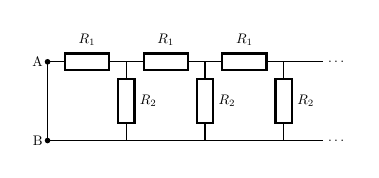
\begin{tikzpicture}[scale=0.5, transform shape]
    % Draw rails and rungs
    \draw (0,2) to[R, l=$R_1$] (2,2) to[R, l=$R_1$] (4,2) to[R, l=$R_1$] (6,2);
    \draw (0,0) -- (2,0) -- (4,0) -- (6,0);
    \draw (2,2) to[R, l=$R_2$] (2,0);
    \draw (4,2) to[R, l=$R_2$] (4,0);
    \draw (6,2) to[R, l=$R_2$] (6,0);
    
    % Draw terminals
    \draw (0,2) -- (0,0);
    \draw (0,2) node[left] {A} node[circ] {};
    \draw (0,0) node[left] {B} node[circ] {};
    
    % Draw continuation dots
    \draw (6,2) -- (7,2) node[right] {$\dots$};
    \draw (6,0) -- (7,0) node[right] {$\dots$};
\end{tikzpicture}
\end{center}

Find the total equivalent resistance $R_{\text{eq}}$ as measured across the input terminals A and B.

\subsubsection*{Solution 2: The Infinite Resistor Ladder}

\begin{enumerate}
    \item \textbf{Identify Self-Similarity:} Let $R_{\text{eq}}$ be the equivalent resistance of the entire infinite ladder. Because the ladder is infinite, if we cut off the first section (the first $R_1$ and $R_2$), the remaining infinite ladder \textit{also} has an equivalent resistance of $R_{\text{eq}}$.
    
    \item \textbf{Set up the Equation:} We can redraw the circuit as the first $R_1$ in series with the parallel combination of the first $R_2$ and the rest of the ladder ($R_{\text{eq}}$).
    \begin{itemize}
        \item Resistance of the parallel part: $R_p = R_2 \parallel R_{\text{eq}} = \frac{R_2 R_{\text{eq}}}{R_2 + R_{\text{eq}}}$
        \item The total resistance, which must be $R_{\text{eq}}$, is $R_1$ in series with $R_p$:
            $$R_{\text{eq}} = R_1 + R_p = R_1 + \frac{R_2 R_{\text{eq}}}{R_2 + R_{\text{eq}}}$$
    \end{itemize}
    
    \item \textbf{Solve for $R_{\text{eq}}$:} This is a quadratic equation.
    \begin{itemize}
        % ... [Algebra steps]
        \item Subtract $R_2 R_{\text{eq}}$ from both sides and rearrange:
            $$R_{\text{eq}}^2 - R_1 R_{\text{eq}} - R_1 R_2 = 0$$
        \item Use the quadratic formula $R_{\text{eq}} = \frac{-b \pm \sqrt{b^2 - 4ac}}{2a}$:
            $$R_{\text{eq}} = \frac{-(-R_1) \pm \sqrt{(-R_1)^2 - 4(1)(-R_1 R_2)}}{2(1)}$$
            $$R_{\text{eq}} = \frac{R_1 \pm \sqrt{R_1^2 + 4 R_1 R_2}}{2}$$
    \end{itemize}
    
    \item \textbf{Choose the Physical Solution:} Since resistance must be a positive value, we take the positive root.
\end{enumerate}
\textbf{Solution: $R_{\text{eq}} = \frac{R_1 + \sqrt{R_1^2 + 4 R_1 R_2}}{2}$}

\hrulefill

% The content of Equvalent_RC_network.tex ends here in the fetched snippet.

\newpage

%%%%%%%%%%%%%%%%%%%%%%%%%%%%%%%%%%%%%%%%%%%%%%%%%%%%%%
%
% FILE 3: Capacitor_problem.tex
%
%%%%%%%%%%%%%%%%%%%%%%%%%%%%%%%%%%%%%%%%%%%%%%%%%%%%%%

\section*{New Problems: Capacitors}

Here are three new problems designed to test the same core concepts of capacitor networks, dielectrics, and AC circuits, complete with detailed explanations and solutions.

\subsection{Problem 1: The Alternative Infinite Ladder}
\noindent\textbf{Question:} An infinite capacitor ladder, constructed with capacitors of $C = \SI{2.0}{\micro\farad}$, is connected to a \SI{100}{\volt}, \SI{60}{\hertz} AC power supply. What is the RMS current drawn from the supply?

\begin{figure}[htbp]
\centering
\begin{circuitikz}[scale=1]
    \draw (0,0) to[sV, l=\SI{100}{V} \SI{60}{Hz}] (0,2.5)
          to[ammeter] (1.5,2.5)
          to[C, l=$C$] (3.5,2.5);
    \draw (3.5,2.5) -- (3.5,1.5) to[C, l=$C$, mirror] (3.5,0);
    \draw (3.5,2.5) to[C, l=$C$] (5.5,2.5);
    \draw (5.5,2.5) -- (5.5,1.5) to[C, l=$C$, mirror] (5.5,0);
    \draw (5.5,2.5) to[C, l=$C$] (7.5,2.5);
    \draw (7.5,2.5) -- (7.5,1.5) to[C, l=$C$, mirror] (7.5,0);
    \draw (0,0) -- (7.5,0);
    \draw[dashed, thick, ->] (7.5,2.5) -- (8.5,2.5);
    \draw[dashed, thick, ->] (7.5,0) -- (8.5,0);
    \node[align=center] at (8.5,1.25) {Repeat to \\ infinity...};
\end{circuitikz}
\caption{The infinite L-C ladder network.}
\end{figure}

\subsubsection*{Explanation & Solution}
\begin{enumerate}
    \item \textbf{Set up the Self-Similarity Equation:}
    Let the equivalent capacitance be $C_{eq}$.
    The circuit is equivalent to one capacitor $C$ in series with the parallel combination of another capacitor $C$ and the rest of the ladder ($C_{eq}$).
    $$ C_{eq} = \left( \frac{1}{C} + \frac{1}{C + C_{eq}} \right)^{-1} $$
    $$ \frac{1}{C_{eq}} = \frac{1}{C} + \frac{1}{C + C_{eq}} $$
    
    \item \textbf{Solve for $C_{eq}$:}
    Rearrange into a quadratic equation:
    % ... [Algebra steps]
    $$ C_{eq}^2 + C C_{eq} - C^2 = 0 $$
    Using the quadratic formula, and taking the positive root for capacitance:
    $$ C_{eq} = \frac{-C + \sqrt{C^2 - 4(1)(-C^2)}}{2} = C \left( \frac{\sqrt{5}-1}{2} \right) $$
    Given $C = \SI{2.0}{\micro\farad}$:
    $$ C_{eq} = (\SI{2.0e-6}{\farad}) \left( \frac{2.236 - 1}{2} \right) \approx \SI{1.236e-6}{\farad} $$

    \item \textbf{Calculate Capacitive Reactance ($X_C$):}
    $$ X_C = \frac{1}{2\pi f C_{eq}} = \frac{1}{2\pi (\SI{60}{\hertz})(\SI{1.236e-6}{\farad})} \approx \SI{2146}{\ohm} $$

    \item \textbf{Calculate the RMS Current ($I_{rms}$):}
    $$ I_{rms} = \frac{V_{rms}}{X_C} = \frac{\SI{100}{\volt}}{\SI{2146}{\ohm}} \approx \SI{0.0466}{\ampere} $$
\end{enumerate}
\textbf{Answer:} The RMS current drawn from the supply is \textbf{\SI{46.6}{mA}}.

\newpage

\subsection{Problem 2: Dielectric Insertion (Constant Charge)}
\noindent\textbf{Question:} A parallel plate capacitor with capacitance $C = \SI{10}{\micro\farad}$ is charged by a \SI{12}{\volt} battery.
The battery is then disconnected. Afterwards, a dielectric slab with a dielectric constant $\kappa = 4.0$ is inserted, completely filling the space between the plates.
What is the final voltage across the capacitor and the final energy stored?

\begin{figure}[htbp]
\centering
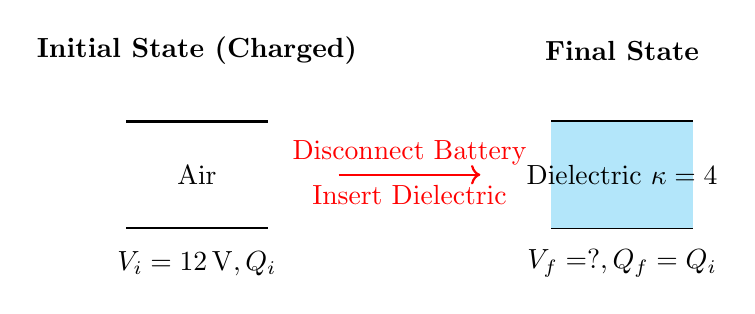
\begin{tikzpicture}[scale=0.9]
    % Initial State
    \node at (0, 2.5) {\textbf{Initial State (Charged)}};
    \draw[thick] (-1,0) -- (1,0);
    \draw[thick] (-1,1.5) -- (1,1.5);
    \node at (0, 0.75) {Air};
    \node at (0, -0.5) {$V_i = \SI{12}{\volt}, Q_i$};
    \draw[->, thick, red] (2, 0.75) -- (4, 0.75) node[midway, above] {Disconnect Battery} node[midway, below] {Insert Dielectric};
    % Final State
    \node at (6, 2.5) {\textbf{Final State}};
    \draw[thick] (5,0) -- (7,0);
    \draw[thick] (5,1.5) -- (7,1.5);
    \fill[cyan!30] (5,0) rectangle (7,1.5);
    \node at (6, 0.75) {Dielectric $\kappa=4$};
    \node at (6, -0.5) {$V_f = ?, Q_f = Q_i$};
\end{tikzpicture}
\caption{Process of inserting a dielectric with the battery disconnected.}
\end{figure}

\subsubsection*{Explanation & Solution}
\begin{enumerate}
    \item \textbf{Calculate the Initial Charge ($Q$):}
    When connected to the battery, the capacitor stores a charge $Q$.
    After disconnection, this charge is trapped and remains constant.
    $$ Q = C_i V_i = (\SI{10e-6}{\farad})(\SI{12}{\volt}) = \SI{120e-6}{\coulomb} = \SI{120}{\micro\coulomb} $$

    \item \textbf{Calculate the Final Capacitance ($C_f$):}
    Inserting the dielectric increases the capacitance by a factor of $\kappa$.
    $$ C_f = \kappa C_i = (4.0)(\SI{10}{\micro\farad}) = \SI{40}{\micro\farad} $$
    
    % ... [Rest of solution from file]
\end{enumerate}

% The content of Capacitor_problem.tex ends here in the fetched snippet.


\end{document}